\documentclass[letterpaper]{article}

\usepackage{natbib,alifeconf,amsmath,listings,subcaption,textcomp,url,xcolor, flushend}  %% The order is important - natbib must be before alifeconf

% Automatic formatting of SI units
\usepackage[binary-units]{siunitx}

% Configure listing
\lstset{language=C++,showstringspaces=false,upquote=true,identifierstyle=\ttfamily\color{black}}

% Visible TODO notes
\newcommand{\todo}[1]{\textbf{\textsc{\textcolor{red}{(TODO: #1)}}}}

\title{Insect-Inspired Visual Navigation On-Board an Autonomous Robot:\\ Real-World Routes Encoded in a Single Layer Network}
%\title{Insect-Inspired Route Navigation On-board an Autonomous Robot}
\author{James C. Knight$^{1}$, Daniil Sakhapov$^{2}$, Norbert Domcsek$^{1}$, Alex Dewar$^{1}$,\\ 
{\Large Paul Graham$^{1}$, Thomas Nowotny$^{1}$ \and Andrew Philippides$^{1}$} \\
\mbox{}\\
$^1$Centre for Computational Neuroscience and Robotics, University of Sussex, Brighton, UK \\
$^2$Department of Computer Science, Tomsk State University, Tomsk, Russia \\
J.C.Knight@sussex.ac.uk} % email of corresponding author

% For several authors from the same institution use the same number to
% refer to one address.
%
% If the names do not fit well on one line use
%         Author 1, Author 2 ... \\ {\Large\bf Author n} ...\\ ...
%
% If the title and author information do not fit in the area
% allocated, place \setlength\titlebox{<new height>} after the
% \documentclass line where <new height> is 2.25in



\begin{document}
\maketitle

\begin{abstract}
% Abstract length should not exceed 250 words
Inspired by the behaviour of ants, models of visually-guided navigation that operate by scanning for previously experienced views of the world have been shown to be capable of robust route navigation. 
These algorithms operate by training an artificial neural network~(ANN) to output a measure of the familiarity of any view after training  with the views experienced along a training route.
Hence we refer to them as familiarity-based navigation algorithms.
In this paper we show that an ANN with an Infomax learning rule is capable of delivering reliable direction information, even when scenes contain few local landmarks and high-levels of noise (from changing lighting conditions, uneven terrain etc). 
Indeed, routes can be precisely recapitulated, with our robot straying an average of only \SI{10}{\centi\metre} from the \SI{6}{\metre} training path. 
Additionally, we show that the required computation does not increase with the number of training views and thus the ANN provides a compact representation of the knowledge needed to traverse a route. 
Finally, rather than this compact representation necessarily losing information, there are instances where the use of an ANN ameliorates the problems of sub-optimal paths caused by very tortuous training routes. 
Our results therefore suggest the feasibility of familiarity-based navigation for long-range autonomous visual homing.
\end{abstract}

\section{Introduction}
Visual homing -- the ability to navigate back to a place of interest using visual information alone -- is a problem of great interest for both engineers seeking to build autonomous robots and neuroethologists seeking to understand its neural basis in animals~\citep{Graham2014}.
In the animal kingdom, solitary foraging ants are one of the champion visual navigators~\citep{Wehner2009}.
Despite having small brains and low resolution vision, these ants can learn visually guided routes many metres long through complex terrain~\citep{Knaden2016}.o
However, in direct contrast with most modern robotic methods, to navigate between two locations, insects use route knowledge not mental maps~\citep{Wehner2006}. 
That is, insects learn procedural instructions for navigation: ``What should I do here?'' rather than ``Where am I?''. 
This allows for much simpler mental representations of the visual world with corresponding potential for computational efficiencies.
We have shown that route knowledge can be learnt and represented holistically using an artificial neural network (ANN)~\citep{Philippides2015}, without specifying when or what to learn~\citep{Baddeley2011} and from a single exposure to the route data~\citep{Baddeley2012}. 
One of the reasons to use an ANN is that route knowledge can be encoded and used with memory and computational constraints that do not scale with route length, are plausible for an ant and, as a corollary, well-suited to a small, power-efficient, robot. 
In this paper we therefore explore how well a single layer ANN can guide a small robot through real world routes of up to \SI{10}{\metre} with all compution being performed on-board.
%While these algorithms have been extensively tested in simulations of complex ant habitats, there has been no previous investigation into how an ANN-based route encoding would function in the real world. 
%In this paper we explore the performance of our familiarity-based algorithm -- in which routes are encoded in a single layer network trained with an (unsupervised) Infomax training rule -- running on-board an autonomous robot and recapitulating routes of up to \SI{10}{\metre}. 

Our route navigation algorithms start with two observations. 
Firstly, if an agent stores a view when facing a given direction, the difference between it and views from a nearby location, but at a range of headings, will be minimised when the agent is facing the same direction as when the first image was stored~\citep{Zeil2003}. 
Secondly, for ants and many wheeled robots, there is a fixed relationship between viewing direction and direction of travel, meaning that a view implicitly defines a movement direction.
Therefore, when an agent is facing in a familiar direction, it is likely travelling in the correct direction. 
This allows the problem of navigation to be reframed in terms of a search for familiar views, that is, views that are associated with a previously learned route.
Based on this, we have developed a parsimonious insect-inspired navigation algorithm in which a route, or routes, are learnt holistically and route recapitulation is driven by a search for familiar views~\citep{Baddeley2012}.

The algorithm proceeds as follows: an agent equipped with a low-resolution \SI{360}{\degree} panoramic visual sensor first travels a route.
The views it experiences along this route -- crucially determined by both the agent’s positions and headings (poses) -- are used to sequentially train an artificial neural network~(ANN) which learns a holistic representation of the views encountered. Subsequently, the network is used to estimate the likelihood of whether a given view -- and thus a pose -- has been experienced before.
When trying to repeat the route, the agent derives a direction of movement at a position by visually scanning the environment (either by physically rotating -- a behaviour seen in ants~\citep{Wystrach2014} -- or rotating the view `in silica').
Each rotated version of the current view is applied as an input to the network which outputs an estimate of its familiarity.
The agent then moves in the direction corresponding to the view most similar to those encountered during learning.

Algorithms of this sort have been used to successfully learn routes through simulations of the habitats of solitary foraging ants, using a variety of neural networks as the route encoding, ranging from restricted Boltzmann machines~\citep{Baddeley2011models} to a spiking model of part of an ant’s brain known as the mushroom body~\citep{Ardin2016}.
The paths of these simulated agents have then been shown to demonstrate many of the characteristics of the paths of ants~\citep{Wystrach2013}.
Here, we follow \citet{Baddeley2012} who showed that a single layer network trained with an Infomax learning rule can not only navigate robustly, but can learn multiple paths to a single goal in a single trial with performance robust to sensor and motor noise.
We choose to use this approach mainly because it only requires a single pass through the data, meaning that each view is experienced just once and then discarded.
While the parsimony of encoding and recall makes this algorithm suitable for use on a small autonomous robot, it had not previously been tested in the real world.
Here, we show that the robot shown in Figure~\ref{fig:robot} can navigate fully autonomously outdoors using only a single layer neural network, with all processing performed on-board the robot using a Jetson TX1~\citep{NVIDIACorporation2016}.
%In particular we investigate whether the compact encoding loses useful information and show that instead, it can geenralis

\begin{figure}[t]
    \centering
    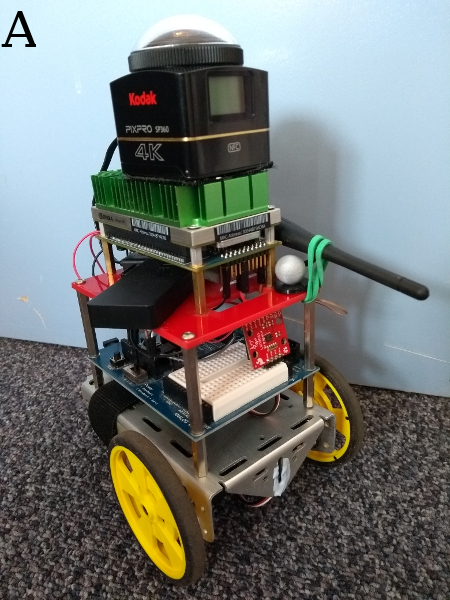
\includegraphics[height=2in]{figures/robot.jpg}
    \caption{Robot platform with onboard computation.}
    \label{fig:robot}
\end{figure}

\section{Methods}
As described above, at the heart of our algorithm an agent navigates by sampling views from the current position at a number of headings and finding the direction that is deemed most familiar by comparison to the views perceived during a training route. 
We find this most familiar direction in two ways. 
Firstly, we train a neural network to output the familiarity of the training views and input rotated versions of the current view to it. 
This results in a rotational familiarity function (RFF -- Figure~\ref{fig:good_ridf}) which, for each heading faced, gives a familiarity score.
The heading with the highest score is the most familiar and sets the movement direction taken.
Secondly, as a baseline and because it allows easier interpretation of the data (for instance, to identify points in routes that are easy/hard or contain misleading information) we also implement what we previously termed the Perfect Memory model. 
In this variant, the rotated current views are compared directly in a pixel-wise manner to every training view in turn (which would not be plausible for an ant). 
In the following sections we first describe the perfect memory algorithm before describing the ANN and Infomax learning rule.

\begin{figure}[t]
    \centering
    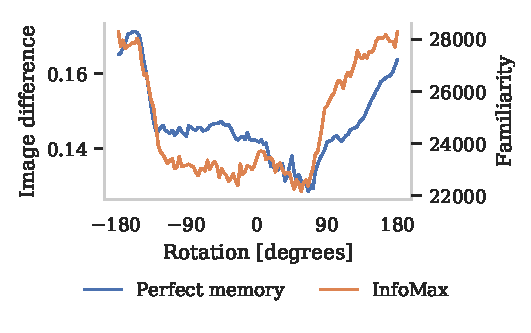
\includegraphics{figures/good_ridf.eps}
    \caption{Example Rotational Image Difference Function~(RIDF) from Perfect memory algorithm and Rotational Familiarity Function~(RFF) from InfoMax.}
    \label{fig:good_ridf}
\end{figure}

\begin{figure*}[t]
    \centering
    \begin{subfigure}[b]{\columnwidth}
        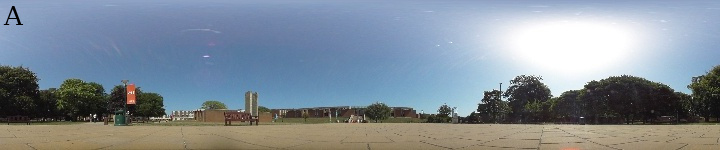
\includegraphics[width=\columnwidth]{figures/360_240.jpg}
    \end{subfigure}
    \begin{subfigure}[b]{\columnwidth}
        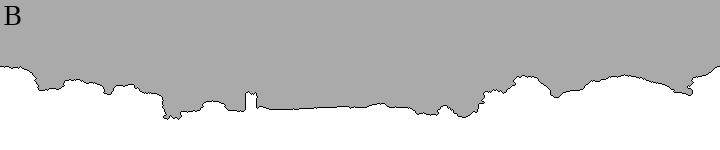
\includegraphics[width=\columnwidth]{figures/360_240_mask.png}
    \end{subfigure}
    \caption{Example panoramic images from our database.
    \textbf{A} Raw unprocessed image.
    \textbf{B} Sky-segmented binary image.}
    \label{fig:database_images}
\end{figure*}

\subsection{Route navigation with a perfect memory}
\label{sec:ridf_perfect_memory}
In our `perfect memory' version of the algorithm, each rotated view is sequentially compared to all of the training views. 
The best matching heading is then defined as the one with the lowest image difference, across all training views and rotations. 
Image difference can be calculated by various functions but here we use the average absolute difference between each of the image pixels to calculate the Image Difference Function~(IDF):
%
\begin{align}
    IDF\Bigl(C(\vec{a}, \theta), S(\vec{b}, \phi)\Bigr) = \frac{1}{p \times q} \sum\limits_{i=1}^p{\sum\limits_{j=1}^q|{C_{i,j} - S_{i,j}|}}
\end{align}
%
where $C(\vec{a}, \theta)$ is a $p \times q$ pixel view captured at location $\vec{a}$ with heading $\theta$; $S(\vec{b}, \phi)$ is a $p \times q$ pixel snapshot stored in memory; and $C_{i,j}$ and $S_{i,j}$ refers to the intensity of pixels in row $i$ and column $j$ of the captured view and stored snapshot respectively.
A Rotational Image Difference Function~(RIDF) is thus generated by varying theta through a range of angles and calculating the IDF at each rotation. 
Where there is a good match, there will be a minimum in the RIDF which defines the best matching direction. 
An example RIDF is shown in Figure~\ref{fig:good_ridf} which has a clear minimum at the best matching heading of around \SI{60}{\degree}.
As the RIDF will also have minima at other matching headings, we can use this to, for example, analyse locations where there has been a bad match to see whether it is the result of visual aliasing.

\begin{figure*}[t]
    \centering
    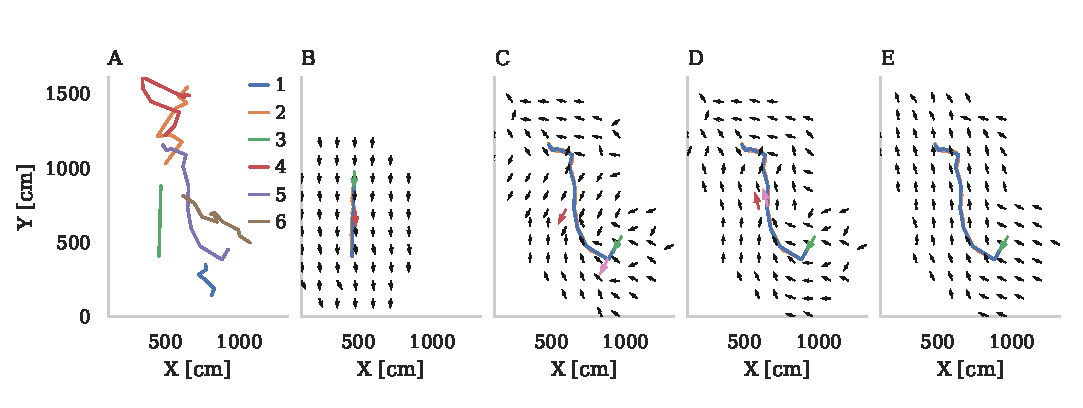
\includegraphics{figures/vector_field.eps}
    \caption{Vector fields showing the directions an agent, trained on a route, would move at each point within \SI{4}{\metre} of the route using a Perfect Memory algorithm with the skyline extracted using the watershed algorithm. 
    Orange lines shows data from our camera-based tracking of the robot and blue lines show the version simplified using the Ramer-Douglas-Peucker algorithm~\citep{Ramer1972}.
    Green arrows indicate the position and direction the robot starts at.
    Red and pink arrows indicate positions in the vector field referred to in later analysis.
    \textbf{A} Simple route (route 3).
    \textbf{B} Longer route (route 5) where visual aliasing occurs in the middle section.
    \textbf{C} By only considering rotated views within \SI{90}{\degree} of the route, visual aliasing problems can be avoided in route 5.
    \textbf{D} Using InfoMax, tortuous elements of route 5 are smoothed out in the vector field.}
    \label{fig:vector_fields}
\end{figure*}

\subsection{Familiarity-based route navigation}
\label{sec:familiarity_infomax}
To perform familiarity discrimination we follow \citet{Baddeley2012} and use a neural network model that was specifically designed to perform this task~\citep{Lulham2011}. 
The architecture consists of an input layer and a novelty layer with $tanh()$ activation functions. 
The number of input units is equal to the dimensionality of the input which in our case is $[120 \times 25]=3000$, the number of pixels in a down-sampled view of the world. 
The number of novelty units is arbitrary and here we use the same number of novelty units as inputs although, using fewer novelty units has worked in simulation and will be tested in future work.
%We found that using as few as \num{200} novelty units can work well in many instances, but we do not explore this aspect of the problem as we were more interested in the behavioural consequences of a familiarity driven approach. 
The network is fully connected by feedforward connections $w_{ij}$. 
Weights are initialised randomly from a uniform distribution in the range $[-0.5,0.5]$ and then normalised so that the mean of the weights feeding into each novelty unit is \num{0} and the standard deviation is \num{1}. 
The network is then trained using the Infomax principle~\citep{Bell1995}, adjusting the weights so as to maximise the information that the novelty units provide about the input, by following the gradient of the mutual information using Equation~\ref{eqn:infomax_learning} which performs gradient ascent using the natural gradient~\citep{Amari1998} of the mutual information over the weights~\citep{Lee1997}
During learning the activation of each of the $M$ novelty units $h_{i}$ is computed as:
%
\begin{align}
    h_{i}=\sum\limits_{j=1}^N w_{ij}x_{j}   \label{eqn:infomax_activation}
\end{align}
%
where $x_{j}$ is a row vector assembled by concatenating the rows of $C(\vec{a}, \theta)$ and $N=p \times q$~(the number of input units).
The output $y_{i}$ of the novelty units is then given by:
%
\begin{align}
    y_{i}=tanh(h_{i})   \label{eqn:infomax_output}
\end{align}
%
The weights are then adjusted using the following learning rule: 
%
\begin{align}
    \Delta w_{ij}=\frac{\eta}{N} \Bigl( w_{ij} - (y_{i} + h_{i}) \sum\limits_{k=1}^N h_{k}w_{kj} \Bigr)   \label{eqn:infomax_learning}
\end{align}
%
where $\eta$ is the learning rate and is set as \num{0.01} for this paper. 
Finally, the response of the network to the presentation of an unseen N-dimensional input $\vec{x}$ is computed as
%
\begin{align}
    \text{fam}(\vec{x})=\sum\limits_{i=1}^N |h_{i}|     \label{eqn:infomax_response}
\end{align}
%
where $||$ denotes the absolute value.
By applying $C(\vec{a}, \theta)$ to the ANN for a range of $\theta$, an RFF can be calculated from $\text{fam}(\vec{x})$.

\subsection{Robot platform}
\label{sec:robot_platform}
In this work we use the robot platform developed by \citet{Domcsek2018} shown in Figure~\ref{fig:robot}.
This robot is based on a Parallax `Shield-Bot' chassis~\citep{ParallaxInc}, with a Jetson TX1 embedded computer~\citep{NVIDIACorporation2016} mounted on top for additional onboard computation and additional batteries mounted underneath. 
The Jetson TX1 is connected via USB to a Kodak PixPro SP360 4K camera~\citep{JKImagingLtd}, mounted on top of the robot connected which provides panoramic visual input.

\subsection{Image processing and data collection}
\label{sec:image_database}
Using a Kodak PixPro SP360 4K panoramic camera~\citep{JKImagingLtd}, we recorded \num{195} images of the ‘Library Square’ at the University of Sussex. 
These were taken on a \SI{1.2}{\metre} grid, aligned with the slabs the square is paved with.
As well as this reference grid of images, we also recorded videos from the same camera mounted on the mobile robot described in the previous section, as we manually drove it along six routes of varying lengths and tortuosity across the square. 
We tracked the robot by using the Discriminative Correlation Filter Tracker with Channel and Spatial Reliability~\citep{Lukezic2018} implementation provided by OpenCV~\citep{OpenCV} to extract the position of the robot over time from video captured by a tripod-mounted camera. 
Finally, we used OpenCV to apply a perspective transform to the positions extracted by the tracker and married these final positions with the video frames captured by the robot. 

As it has previously been shown that the sky can give erroneous information for visual homing and that visual homing can in fact be achieved using a binary image consisting of sky/not-sky~\citep{Philippides2011,Stone2014} -- we wanted to compare the use of raw and binary images.
To achieve this in real-time on the robot, we used the watershed segmentation algorithm~\citep{Beucher1979} with markers placed at the top and bottom of each image.
Figure~\ref{fig:database_images} shows some example images from this database.

\begin{figure}[t]
    \begin{subfigure}[b]{\columnwidth}
        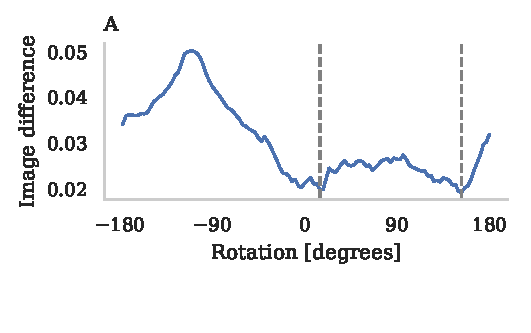
\includegraphics[width=\columnwidth]{figures/alias_ridf.eps}
    \end{subfigure}
    \begin{subfigure}[b]{\columnwidth}
        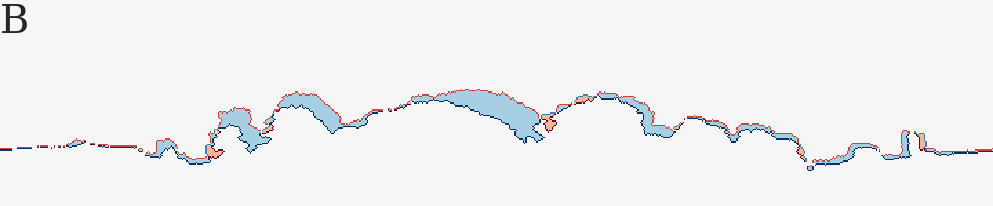
\includegraphics[width=\columnwidth]{figures/image_diff_bad.png}
    \end{subfigure}
    \begin{subfigure}[b]{\columnwidth}
        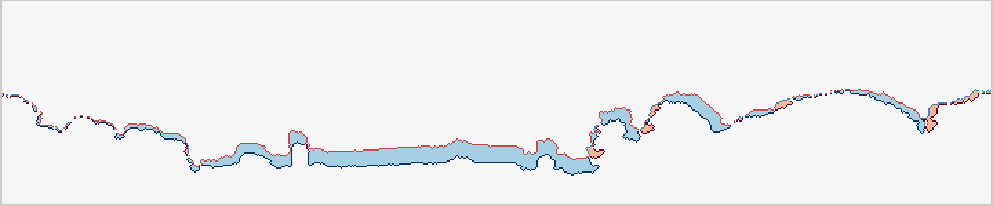
\includegraphics[width=\columnwidth]{figures/image_diff_good.png}
    \end{subfigure}
    \caption{Analysis of aliasing shown in Figure~\ref{fig:vector_fields}b.
    Using grid image taken at location marked with red arrow in Figures~\ref{fig:vector_fields}b~and~\ref{fig:vector_fields}c (\SI{600}{\metre}, \SI{720}{\metre}).
    All images were pre-processed using watershed segmentation algorithm.
    \textbf{A} Rotational Image Difference function.
    \textbf{B} Difference image with visual aliased route image found at location marked with pink arrow in Figure~\ref{fig:vector_fields}b.
    \textbf{C} Difference image with correct route image found at location marked with pink arrow in Figure~\ref{fig:vector_fields}c}
    \label{fig:aliasing}
\end{figure}

\begin{figure}[t]
    \begin{subfigure}[b]{\columnwidth}
        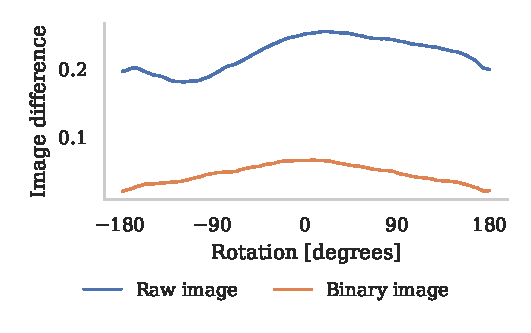
\includegraphics[width=\columnwidth]{figures/route3_ridf.eps}
    \end{subfigure}
    \begin{subfigure}[b]{\columnwidth}
        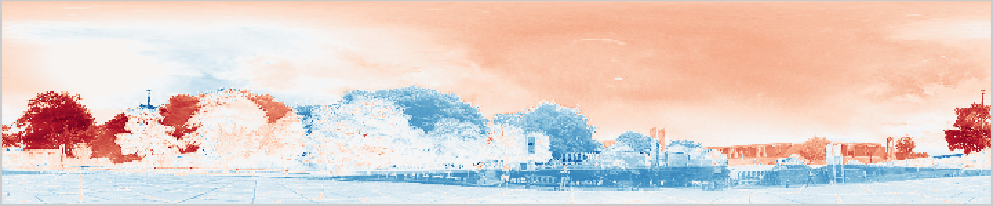
\includegraphics[width=\columnwidth]{figures/route3_unwrapped_image_diff.png}
    \end{subfigure}
    \begin{subfigure}[b]{\columnwidth}
        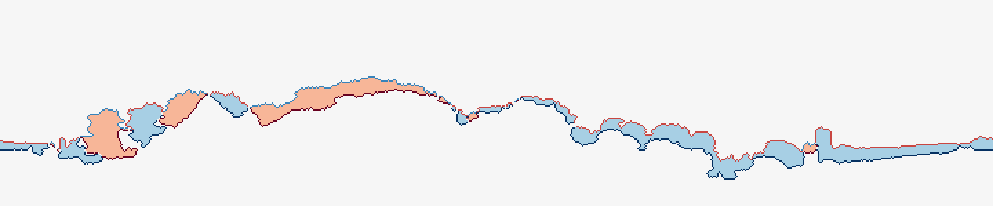
\includegraphics[width=\columnwidth]{figures/route3_mask_image_diff.png}
    \end{subfigure}
    \caption{Analysis of poor performance on route 3 when using raw input images.
    Using grid image taken at location marked with red arrow in figure~\ref{fig:vector_fields}a (\SI{480}{\metre}, \SI{720}{\metre}).
    \textbf{A} Rotational Image Difference function.
    \textbf{B} Difference image based on raw input images.
    \textbf{C} Difference image based on sky-segmented binary input images.}
    \label{fig:light_level}
\end{figure}

\begin{figure*}[t]
    \centering
    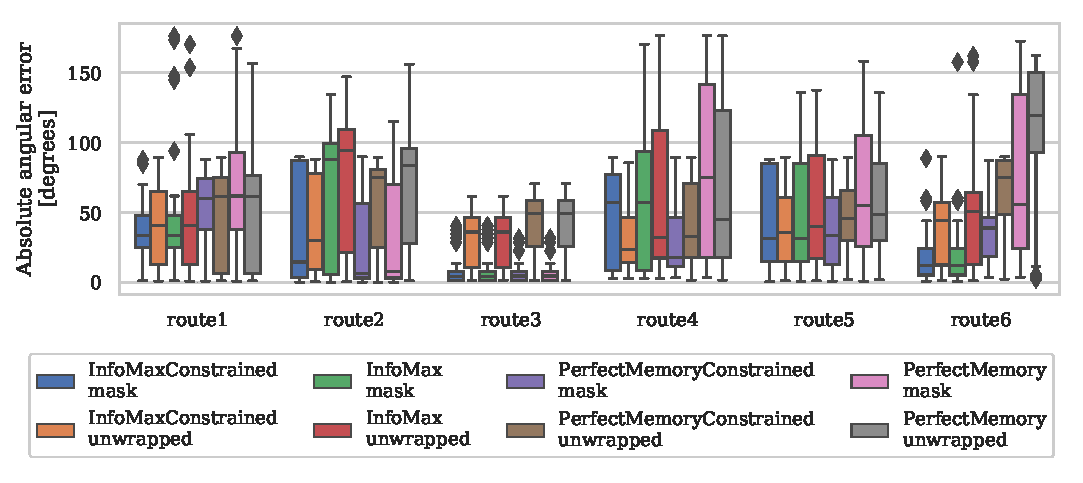
\includegraphics{figures/route_benchmark.eps}
    \caption{Performance of different algorithms on each of the 6 routes.}
    \label{fig:route_benchmark}
\end{figure*}

\section{Results}
\subsection{Offline simulations}
\label{sec:offline_simulations}
We trained both the InfoMax and Perfect Memory algorithms on the images taken along the six routes in our dataset and then used them to find the direction a robot would move when placed at each grid point within \SI{4}{\metre} of the trained route. 
Figure~\ref{fig:vector_fields} shows some example vector fields obtained by plotting this direction at each of the chosen grid locations when using the Perfect Memory algorithm described in Section~\ref{sec:ridf_perfect_memory} with the watershed segmentation-based pre-processing discussed in Section~\ref{sec:image_database}. 
While the vector field suggests that the route shown in Figure~\ref{fig:vector_fields}a would be recapitulated successfully, in the middle section of the route shown in Figure~\ref{fig:vector_fields}b, errors occur.
Figure~\ref{fig:aliasing}a shows a RIDF taken at one of the problematic locations on this route (\SI{600}{\metre}, \SI{720}{\metre}) and it is clear that, as well as the local minima representing the correct heading at \SI{15}{\degree}, there is an additional, slightly lower global minimum at \SI{153}{\degree} which is overriding the correct choice.
Figure~\ref{fig:aliasing} show the per-pixel differences between the best-matching and the closest images (in terms of distance to the current point) taken from training route; and the rotated versions of current image which best match these training images.
Although the \emph{shape} of the skyline in the closest image (Figure~\ref{fig:aliasing}c) is clearly better matched than it is with the best-matching image (Figure~\ref{fig:aliasing}b), there is a vertical offset -- probably caused by camera shake -- which introduces a large difference between the two images.
Therefore the perfect memory model matches the more distant image better and thus the direction taken is similar to the direction taken at this point in the route which results in an error at this location (indicated with a pink arrow in Figure~\ref{fig:vector_fields}b).

However, if we were recapitulating the route using a real robot, these false-positive matches could be eliminated and computation could be saved by simply \emph{not} scanning the full \SI{\pm 180}{\degree} but instead only scanning \SI{\pm 90}{\degree} around the robot's current heading.
However, unlike in the live robot tests, in the database there is no current heading.
We therefore simulated the effect of this modified algorithm using our database of images by simplifying each route using the Ramer-Douglas-Peucker algorithm~\citep{Ramer1972} and calculating the direction of each of the resultant segments.
Each point in the database is then assigned a `current' heading which is equal to the direction of the nearest segment.
Using these headings, we can then ignore matches that would involve heading more than \SI{\pm 90}{\degree} away from the direction of the nearest section of the route and Figure~\ref{fig:vector_fields}c shows that this step solves the aliasing problems in this particular case.
In order to quantify the performance of our algorithms, we used the absolute difference between the most familiar heading angle obtained at each location on the grid and the direction of the nearest route segment as an error measure.
The distributions of these errors across all of the routes, algorithms and image pre-processesing steps is plotted in Figure~\ref{fig:route_benchmark} and shows that, in fact, only scanning \SI{\pm 90}{\degree} improves performance in all cases.
Furthermore, Figure~\ref{fig:route_benchmark} also shows that, when using the Perfect Memory algorithm, sky-segmentation improves performance for almost all routes.
This is particularly noticeable on route 3 (a straight line) where, when using sky-segmented input images, all of the algorithms reconstruct the direction of the route with a very small median error of around \SI{4}{\degree} but, when using unprocessed input images, this increases to around \SI{40}{\degree}.
Figure~\ref{fig:light_level}a shows that, unlike the situation explored earlier in this section, this is not an aliasing problem as there is only a single minima present in each RIDF.
However, the magnitude of the average image differences between the raw images is much larger than that between the sky-segmented images and the minima is located at the incorrect location.
The difference images shown in Figures~\ref{fig:light_level}b~and~\ref{fig:light_level}c suggest that the incorrect position of the minima when comparing the raw images is likely to be due to the large differences in the sky portion of the image due to clouds and the images having been recorded at a different time of day.

After applying sky-segmentation to the input images and only scanning \SI{\pm 90}{\degree} away from the direction of the nearest section of the route, the InfoMax ANN results in a lower median error than the Perfect memory control algorithm in 3 of the 6 routes although this difference is not statistically significant.
Furthermore, if we compare Figures~\ref{fig:vector_fields}c~and~\ref{fig:vector_fields}d, the vector field plotted using the InfoMax ANN appears much smoother, suggesting that rather than losing useful information, the InfoMax encoding may actually be beneficial for smoothing out overly tortuous training routes.

\begin{figure}[t]
    \centering
    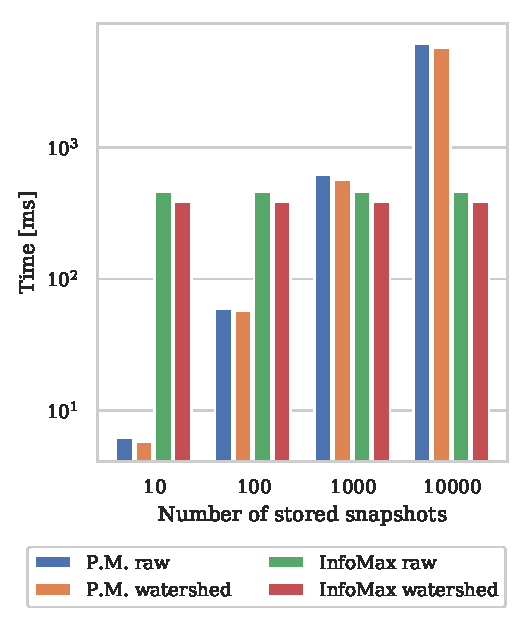
\includegraphics{figures/jetson_test_performance.eps}
    \caption{Performance of visual navigation algorithms running on Jetson TX1. 
    Reported times are measured using \lstinline{std::chrono::high_resolution_clock} and average is taken over \num{100} images.}
    \label{fig:jetson_test_performance}
\end{figure}

\subsection{Computational cost of algorithm}
In the previous section, we showed that the algorithms described in Sections~\ref{sec:ridf_perfect_memory}~and~\ref{sec:familiarity_infomax} are capable of robustly extracting heading direction in outdoor scenes. 
However, in order to deploy these algorithms on a real robot with constrained on board processing, their performance is important. 
In order to measure performance in a controlled scenario, we wrote a benchmarking application which runs on the Jetson TX1 and trains either the Perfect memory or the InfoMax algorithm with varying numbers of images and then measures how long it takes to extract a heading from a testing image (averaged over \num{100} iterations) using \lstinline{std::chrono::high_resolution_clock}.
Figure~\ref{fig:jetson_test_performance} shows the performance of our implementation of the InfoMax algorithm compared to the Perfect memory control using $120 \times 25$ pixel input images.
Clearly, for small numbers of stored images, extracting heading information using the Perfect Memory is faster but, assuming that training images are sampled every \SI{100}{\milli\second}, InfoMax begins to more efficient for routes with only a little over \SI{1}{\minute} of training data making it much more feasible approach for long-range visual homing.

\begin{figure}[t]
    \centering
    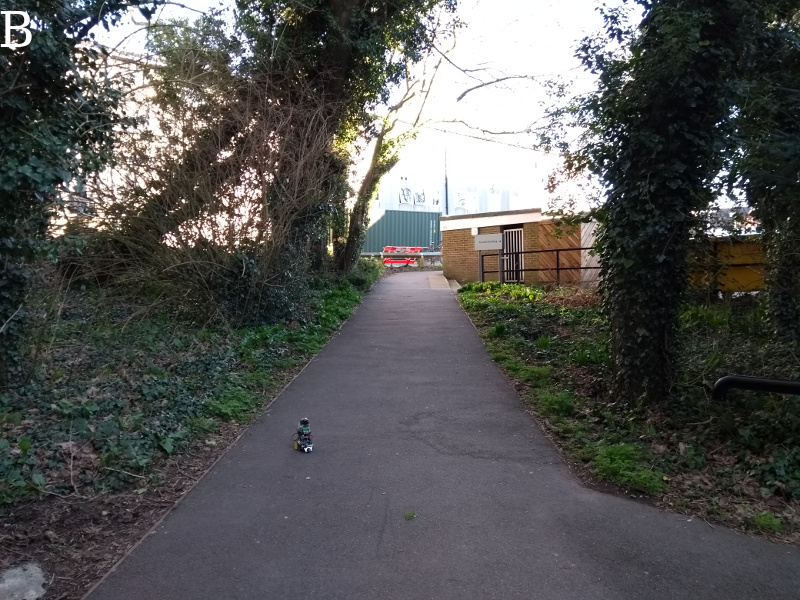
\includegraphics[height=2in]{figures/robot_environment.jpg}
    \caption{Environment used for robot testing.}
    \label{fig:robot_environment}
\end{figure}

\begin{figure}[t]
    \centering
    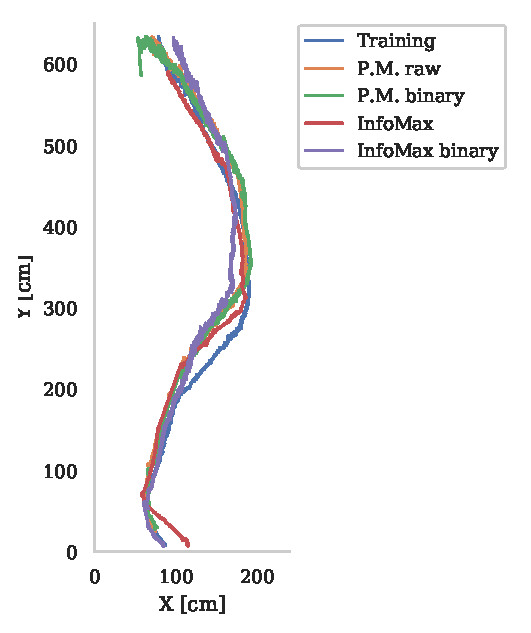
\includegraphics{figures/robot_paths.eps}
    \caption{Reconstructed paths of autonomous robot during training and testing using each algorithm.}
    \label{fig:robot_paths}
\end{figure}

\subsection{Autonomous robot}
Using the implementations of InfoMax and the Perfect Memory algorithms from our Brains-on-Board Robotics library~\citep{Dewar2017}, we built a simple application which can recapitulate learned routes on the robot described in Section~\ref{sec:robot_platform} by running the following simple algorithm every \SI{500}{\milli\second} (based on the performance for 1000 images established in the previous section):
%
\begin{enumerate}
    \item Capture and unwrap a panoramic image.
    \item Perform one of the image processing steps described in Section~\ref{sec:image_database}.
    \item Using either the InfoMax or Perfect Memory algorithm, calculate the familiarity with the processed image ‘in-silico’ when rotated through \SI{\pm 90}{\degree}°.
    \item Find the orientation with the highest familiarity and, if it is within \SI{4}{\degree}, start driving forwards. Otherwise, start turning in the correct direction to align with the image.
\end{enumerate}
%
In order to compare the performance of the navigation algorithms and image processing steps described in Sections~\ref{sec:ridf_perfect_memory},~\ref{sec:familiarity_infomax}~and~\ref{sec:image_database} running on the robot, we first manually drove the robot along a sinuous route through the wooded area shown in Figure~\ref{fig:robot_environment}, recording training images every \SI{100}{\milli\second}.
We then trained each of the navigation algorithms on the resultant dataset of \num{455} images and allowed the robot to recapitulate the path using the procedure described above.
Throughout this training and testing process, we used the method described in Section~\ref{sec:image_database} to track the robot, resulting in the data shown in Figure~\ref{fig:robot_paths}.
The robot was able to successfully recapitulate the training path using each of the navigation and image processing algorithms with little difference in performance immediately apparent in Figure~\ref{fig:robot_paths}.
We confirmed this by calculating the shortest distance to the training path at each location along each recapitulated path and found that, in this environment, there was no significant difference between the performance of the different algorithms and overall the mean of the distance between the training and recapitulated paths was \SI{9}{\centi\metre}, with a standard deviation of \SI{8}{\centi\metre}.

\section{Summary and Discussion}
In this paper we present the first familiarity-based navigation algorithm that can function effectively in the real world on board a small mobile robot using an ANN-based route encoding. 
Indeed, we show that in some cases, using an ANN can improve performance as it imposes a level of generalisation meaning that particularly tortuous elements of the training route (which we presume to be from a noisy training process) are smoothed out in the recapitulated trajectories.

In addition, we reinforce results showing that removing the sky and using only a binary image make these algorithms more robust to variability in lighting and weather conditions~\citep{Philippides2011,Stone2014}. 
Furthermore, these improvements are seen even if the segmentation is performed automatically on board the robot using an RGB image, processed using a simple watershed algorithm rather than requiring specialist sensors such as a UV camera.
Interestingly, these improvements are not noticeable in the results collected using the autonomous robot.
We believe that this is due to the fact that we performed these experiments in a more enclosed environment, where the sky covered a smaller portion of each image and because the testing and training both occurred at the same time of day.
These two factors both act to reduce the differences between the raw images meaning that raw image comparisons are successful.
Additionally, we show that the computation and storage needed to recapitulate a route using the Infomax ANN does not scale with the number of images used in training.
To put this into context of robotic control algorithms, this is not typically a property of SLAM based localization systems where more keyframes are accumulated over time although there has been recent work to cap~\citep{Maddern2012} or at least cull~\citep{Mur-Artal2015} the number of keyframes accumulated.
%While  to the quantity of features features~\citep{Mur-Artal2015}.
%This is not typically a property of SLAM based localization systems where more keyframes are accumulated over time

While visual SLAM implementations based around SURF or SIFT spend several hundred milliseconds extracting features every frame~\citep{Bay2006}, recent SLAM implementations such as FLaME~\citep{Greene2017} have been demonstrated running on autonomous quadrotors at much higher framerates than our current InfoMax implementation can achieve on the Jetson TX1.
However, not only was FLaME implemented on an Intel CPU which \citet{Biddulph2018} measured as being $5\times$ faster than a Jetson TX1, but the performance of our InfoMax algorithm could be significantly improved.
View-based algorithms in general seem to work well with low-resolution wide-field views~\citep{Wystrach2016} and this matches the observation that high-resolution vision in ants is associated with hunting not with long distance navigation~\citep{Wystrach2016}.
Therefore, while $120 \times 25$ pixel images were used throughout the work presented in this paper, \citet{Baddeley2012} first demonstrated InfoMax for visual navigation, they used input images with around half this number of pixels ($90\times 17$). 
Equation~\ref{eqn:infomax_response}  can be implemented as a matrix-vector product -- the computational complexity of which scales quadratically with N. Therefore, using input images with half the number of pixels would quarter the time taken to evaluate Equation~\ref{eqn:infomax_response}. 
Furthermore, while our InfoMax implementation uses OpenMP \todo{ref} to take advantage of the the Jetson TX1's four CPU cores, it does not utilise the \num{256} core GPU present on the Jetson TX1. 
Initial experiments using the cuBLAS~\citep{NVIDIACorporation2007} GPU-accelerated linear algebra library suggest that Equation~\ref{eqn:infomax_response} could be evaluated in around \SI{100}{\milli\second} for $120 \times 25$ pixel images -- a $5 \times$ speedup over our current implementation.
%This paper thus demonstrates the feasibility for efficient rapid learning of visually guided routes for autonomous robots. 
Thus, as with SLAM which has seen vast increases in performance efficiency, further work on the ANN encoding, visual processing and behavioural strategy, will extend the range of homing and reduce computation and training times still further.

\section{Acknowledgements}
This work was funded by the EPSRC (Brains on Board project, grant number EP/P006094/1).

\scriptsize
\bibliographystyle{apalike}
\bibliography{alife} % replace by the name of your .bib file


\end{document}
